% !TeX root = ./ms.tex
\documentclass[modern]{aastex62}

% Load the corTeX style definitions
% !TeX root = ./ms.tex
% All the packages
\usepackage{url}
\usepackage{amsmath}
\usepackage{mathtools}
\usepackage{amssymb}
\usepackage{natbib}
\usepackage{graphicx}
\usepackage{calc}
\usepackage{etoolbox}
\usepackage{xspace}
\usepackage[T1]{fontenc} % https://tex.stackexchange.com/a/166791
\usepackage{textcomp}
\usepackage{ifxetex}
\ifxetex
  \usepackage{fontspec}
  \defaultfontfeatures{Extension = .otf}
\fi
\usepackage{fontawesome}
\usepackage{listings}
\usepackage{nicefrac}
\usepackage[bb=boondox]{mathalfa}
\usepackage{booktabs}
\usepackage{longtable}

% Shorthand for this paper
\newcommand{\starry}{\textsf{starry}\xspace}
\newcommand{\Python}{\textsf{Python}\xspace}
\newcommand{\cpp}{\textsf{C}++\xspace}
\newcommand{\bvec}[1]{{\ensuremath{\mathbf{#1}}}}
\newcommand{\xxx}[1]{{\color{red}#1}}
\DeclarePairedDelimiter\floor{\lfloor}{\rfloor}
\DeclarePairedDelimiter\ceil{\lceil}{\rceil}
\newcommand{\imag}{{\ensuremath{\mathbb{i}}}}
\newcommand{\quadquad}{\quad\quad\quad\quad}

\newcommand{\R}{\bvec{R}}
\newcommand{\AOne}{\bvec{A_1}}
\newcommand{\alm}{\bvec{a}}
\newcommand{\x}{\bvec{x}}
\newcommand{\D}{D}
\newcommand{\Doppler}{\bvec{D}}
\newcommand{\Surf}{\mathcal{S}}
\newcommand{\Curve}{\mathcal{C}}
\newcommand{\Dargs}{\bvec{d}}
\newcommand{\lmax}{\ensuremath{l_\mathrm{max}}}
\newcommand{\spot}{\texttt{SPOT}\xspace}
\newcommand{\vogtstar}{\texttt{VOGTSTAR}\xspace}
\newcommand{\kT}{\boldsymbol{\kappa}^\top}
\newcommand{\rhoT}{\boldsymbol{\rho}^\top}
\newcommand{\ylmbasis}{\boldsymbol{\psi}^\top}
\newcommand{\pbasis}{\boldsymbol{\phi}^\top}
\newcommand{\pbasisn}{\ensuremath{\phi_n}}
\newcommand{\azero}{\ensuremath{\bvec{a_0}}}

% References to text content
\newcommand{\documentname}{\textsl{article}}
\newcommand{\figureref}[1]{\ref{fig:#1}}
\newcommand{\Figure}[1]{Figure~\figureref{#1}}
\newcommand{\figurelabel}[1]{\label{fig:#1}}
\renewcommand{\eqref}[1]{\ref{eq:#1}}
\newcommand{\Eq}[1]{Equation~(\eqref{#1})}
\newcommand{\eq}[1]{\Eq{#1}}
\newcommand{\eqalt}[1]{Equation~\eqref{#1}}

% Add code, proof, and animation hyperlinks
\definecolor{linkcolor}{rgb}{0.1216,0.4667,0.7059}
\newcommand{\codeicon}{{\color{linkcolor}\faFileCodeO}}
\newcommand{\prooficon}{{\color{linkcolor}\faPencilSquareO}}
\newcommand{\codelink}[1]{\href{https://github.com/user/repo/blob/fe12fa16a5cc76c1ba72d97241fb9545da144edf/tex/figures/#1.py}{\codeicon}\,\,}
\newcommand{\animlink}[1]{\href{https://github.com/user/repo/blob/fe12fa16a5cc76c1ba72d97241fb9545da144edf/tex/figures/#1.gif}{\animicon}\,\,}
\newcommand{\prooflink}[1]{\href{https://github.com/user/repo/blob/fe12fa16a5cc76c1ba72d97241fb9545da144edf/tex/proofs/#1.ipynb}{\raisebox{-0.1em}{\prooficon}}}
\newcommand{\cilink}[1]{\href{https://dev.azure.com/user/repo/_build}{#1}}


% Define a proof environment for open source equation proofs
\newtagform{eqtag}[]{(}{)}
\newcommand{\currentlabel}{None}
\newenvironment{proof}[1]{%
  \ifstrempty{#1}{%
    \renewtagform{eqtag}[]{\raisebox{-0.1em}{{\color{red}\faPencilSquareO}}\,(}{)}%
  }{%
    \renewtagform{eqtag}[]{\prooflink{#1}\,(}{)}%
  }%
  \usetagform{eqtag}%
  \renewcommand{\currentlabel}{#1}
  \align%
}{%
  \endalign%
  \renewtagform{eqtag}[]{(}{)}%
  \usetagform{eqtag}%
  \message{<<<\currentlabel: \theequation>>>}%
}

% Display the runtime on Azure
\usepackage[skins]{tcolorbox}
\newtcbox{\figtimebox}{enhanced,nobeforeafter,tcbox raise=-0.8mm,boxrule=0.6pt,
  top=0.5mm,bottom=0mm,right=0mm,left=6mm,arc=1pt,boxsep=2pt,
  before upper={\vphantom{dlg}},colframe=linkcolor,coltext=linkcolor,
  fontupper=\sffamily\bfseries\tiny,colback=white,overlay={\begin{tcbclipinterior}
        \fill[linkcolor] (frame.south west)
        rectangle node[text=white,font=\sffamily\bfseries\tiny,rotate=0]{CPU}
        ([xshift=6mm]frame.north west);\end{tcbclipinterior}}}
\robustify{\figtimebox}
\pdfstringdefDisableCommands{%
  \def\figtimebox#1{'#1'}%
}
\newcommand{\figtime}[1]{\IfFileExists{figures/#1.py.time}%
  {%
    \cilink{\figtimebox{\input{figures/#1.py.time}\unskip s}}
  }{}}

% Define the `oscaption` command for open source figure captions
\newcommand{\oscaption}[2]{\caption{#2 \codelink{#1} \figtime{#1}}}

% Code examples
\definecolor{codegreen}{rgb}{0,0.6,0}
\definecolor{codegray}{rgb}{0.5,0.5,0.5}
\definecolor{codepurple}{rgb}{0.58,0,0.82}
\definecolor{backcolour}{rgb}{0.95,0.95,0.95}
\lstdefinestyle{mystyle}{
  backgroundcolor=\color{backcolour},
  commentstyle=\color{codegreen},
  keywordstyle=\color{magenta},
  numberstyle=\tiny\color{codegray},
  stringstyle=\color{codepurple},
  basicstyle=\small\ttfamily,
  breakatwhitespace=false,
  breaklines=true,
  captionpos=b,
  keepspaces=true,
  numbers=left,
  numbersep=5pt,
  showspaces=false,
  showstringspaces=false,
  showtabs=false,
  tabsize=2,
  aboveskip=1em,
  belowskip=1em,
  keywords=[2]{map},
  keywordstyle=[2]{\color{black!80!black}},
  upquote=true
}
\lstset{style=mystyle}

% Typography obsessions
\setlength{\parindent}{3.0ex}
\renewcommand\quad{\hskip\fontdimen3\font}

% https://tex.stackexchange.com/a/184474
\usepackage{stackengine,scalerel}
\def\lnlam{\ThisStyle{\ensurestackMath{\stackon[-2.4\LMpt]{%
        \SavedStyle\lambda}{\kern-.5pt\kern\LMpt\rule{1\LMex}{.25pt+.15\LMpt}}}}}

% Shorthand for this paper
\usepackage{xifthen}
\newcommand{\BF}[1]{\ensuremath{\mathbf{#1}}}
\newcommand{\BS}[1]{\ensuremath{\boldsymbol{#1}}}
\newcommand{\dd}{\ensuremath{\mathrm{d}}}
\newcommand{\STARRYQUADPOINTS}{100\xspace}
\newcommand{\bkappa}{\BS{\kappa}}
\newcommand{\blambda}{\BS{\lambda}}
\newcommand{\bxi}{\BS{\xi}}
\newcommand{\vmax}{{v_\mathrm{max}}}
\newcommand{\kapint}[1]{%
\sum_{i = 0}^{\frac{N - 1}{2}}
\int\limits_{\frac{1}{2}\kappa_{2i}}^{\frac{1}{2}\kappa_{2i+1}}
#1
\dd\varphi
}
\newcommand{\lamint}[1]{%
\sum_{i = 0}^{\frac{N - 1}{2}}
\int\limits_{\frac{1}{2}\lambda_{2i}}^{\frac{1}{2}\lambda_{2i+1}}
#1
\dd\varphi
}
\newcommand{\coshalfkap}[1][]{%
\ifthenelse{%
    \equal{#1}{}
}{
    \cos\left(\frac{\bkappa}{2}\right)
}{
    \cos^{#1}\left(\frac{\bkappa}{2}\right)
}}
\newcommand{\sinhalfkap}[1][]{%
\ifthenelse{%
    \equal{#1}{}
}{
    \sin\left(\frac{\bkappa}{2}\right)
}{
    \sin^{#1}\left(\frac{\bkappa}{2}\right)
}}
\newcommand{\DE}{\Delta \BS{E}(k^2, \bkappa)}
\newcommand{\DF}{\Delta \BS{F}(k^2, \bkappa)}
\newcommand{\sgn}{{\mathrm{sgn}}}
\newcommand{\xhat}{\ensuremath{\mathbf{\hat{x}}}\xspace}
\newcommand{\yhat}{\ensuremath{\mathbf{\hat{y}}}\xspace}
\newcommand{\zhat}{\ensuremath{\mathbf{\hat{z}}}\xspace}
\newcommand{\sT}{\ensuremath{\BF{s}^\top}}
\newcommand{\rT}{\ensuremath{\BF{r}^\top}}
\newcommand{\bg}{\ensuremath{\tilde{\BF{g}}}}
\newcommand{\bp}{\ensuremath{\tilde{\BF{p}}}}
\newcommand{\by}{\ensuremath{\tilde{\BF{y}}}}

% Bibliography stuff
\bibliographystyle{aasjournal}

% Begin!
\begin{document}

% Title
\title{Analytic Occultation Light Curves in Reflected Light}

% Author list
\author[0000-0002-0296-3826]{Rodrigo Luger}
\email{rluger@flatironinstitute.org}
\affil{Center~for~Computational~Astrophysics, Flatiron~Institute, New~York, NY}
%

\begin{abstract}
    Abstract here.
    %
    \href{https://github.com/rodluger/starrynight}{\color{linkcolor}\faGithub}
\end{abstract}

%
\section{Introduction}
\label{sec:intro}
%
This is an extension of \citet{Luger2019}.

%
\section{The Problem}
\label{sec:the-problem}
%
\subsection{Review of the \starry algorithm in emitted light}
\label{sec:starry-review}
%
Without loss of generality, assume the body whose flux we wish to compute
has radius unity and sits at the origin of a right-handed Cartesian coordinate
system with the $x$-axis pointing to the right on the sky, the $y$-axis
pointing up on the sky, and the $z$-axis pointing out of the sky
toward the observer; denote this frame by $\mathcal{F}_0$. In $\mathcal{F}_0$,
the surface (emitted) intensity field of the body is described by the
spherical harmonic coefficient vector $\mathbf{y}$. Following
\citet{Luger2019}, when no occultor is present, we may compute the total
visible flux $f$ from this body as
%
\begin{align}
    \label{eq:rTA1Ry}
    f = \rT \BF{A_1} \BF{R} \BF{y}
    \quad,
\end{align}
%
where, from right to left, $\BF{R} = \BF{R}(i, \lambda, \vartheta)$
is a Wigner rotation matrix that rotates $\bvec{y}$ to the sky frame
$\mathcal{F}_\mathrm{sky}$ given the body's inclination $i$, obliquity
$\lambda$, and rotational phase $\vartheta$,
%
$\BF{A_1}$ is the change-of-basis matrix from the spherical harmonic
basis $\by$ to the \emph{polynomial basis} $\bp$ in which the integrals
are computed,
%
and $\rT$ is the vector of solutions to the integral over
the projected visible disk of the body for each term in $\bp$.
%
If an occultor is present, we instead compute the visible flux from
%
\begin{align}
    \label{eq:sTARRy}
    f = \sT \BF{A} \BF{R}' \BF{R} \BF{y}
    \quad,
\end{align}
%
where, as before, $\BF{R}$ rotates the body from $\mathcal{F}_0$
to $\mathcal{F}_\mathrm{sky}$,
%
$\BF{R}'$ rotates the body on the plane
of the sky into the frame $\mathcal{F}_\mathrm{greens}$ in which the
integration is actually performed,
%
$\BF{A}$ is the change-of-basis matrix from $\by$
to the \emph{Green's basis} $\bg$ in which the integrals are computed,
%
and $\sT$ is the vector of solutions to the integral over
the projected visible disk of the body for each term in $\bg$.
For more details, see Appendix~\ref{app:starry} and \citet{Luger2019}.

\subsection{Adapting the algorithm to the reflected light case}
\label{sec:starry-review}
%
In order to compute light curves in reflected light, we must make two
modifications to the \starry algorithm. First,
the expressions above assume that the coefficient vector
$\mathbf{y}$ describes the \emph{emissivity} of the body, which (in the
absence of limb darkening) is assumed to be Lambertian, i.e., all points on the
surface emit equally in all directions.
Here, we wish to derive the solution for the flux in the case of Lambertian
reflectance, in which case the vector $\mathbf{y}$ is taken to describe the
surface \emph{reflectivity} (or \emph{Bond albedo}).

Second, we must explicitly model the illumination of the body. We assume the
body is illuminated by a point-like source, in which case the radiance at any
point on the surface is proportional to the cosine of the angle $\phi$ between
the incident light and the surface normal. Points for which
$\phi \ge \frac{\pi}{2}$ are unilluminated and therefore have radiance of zero.
%
If the point-like illumination source is placed at sky coordinates
$(x_s, y_s, z_s)$, the day/night terminator on the body is a half-ellipse
of semi-major axis unity that is fully described by its semi-minor axis,
%
\begin{proof}{}
    \label{eq:b}
    b = -\frac{z_s}{\sqrt{x_s^2 + y_s^2 + z_s^2}}
    \quad,
\end{proof}
%
and the angle by which its semi-major axis is rotated away from the
$+x$-axis,
%
\begin{proof}{}
    \label{eq:theta}
    \theta = \mathrm{arctan2}(y_s, x_s)
    \quad.
\end{proof}
%
Given this formulation, and assuming that
$x_s^2 + y_s^2 + z_s^2 \gg 1$,
it is straightforward to show that the illumination
$I$ at a point $(x, y)$ on the projected disk of the body is given by
the polynomial
%
\begin{proof}{}
    \frac{I(b, \theta; x, y)}{I_0} &=
    -b_c\sin\theta x + b_c\cos\theta y - bz(x, y)
\end{proof}
%
where $b_c = \sqrt{1 - b^2}$, $z(x, y) = \sqrt{1 - x^2 - y^2}$, and
%
\begin{proof}{}
    I_0 = \frac{L}{4\pi\left(x_s^2 + y_s^2 + z_s^2\right)}
\end{proof}
%
is the peak illumination (at the substellar point,
assuming the illumination source is a star), with $L$ equal to the luminosity
of the source.
%
Since the illumination is just a polynomial in $x$, $y$, and $z(x, y)$, we
can express it as a vector $\BF{i}(b, \theta)$ in the polynomial basis $\bp$.
Recalling the structure of the basis (c.f. Appendix~\ref{app:starry}),
%
\begin{align}
    \bp & =
    \begin{pmatrix}
        1   &
        x   & z  & y  &
        x^2 & xz & xy & yz & y^2 &
        \cdot\cdot\cdot
    \end{pmatrix}^\mathsf{T}
    \quad,
\end{align}
%
we may write
%
\begin{proof}{}
    \BF{i}(b, \theta) & =
    I_0
    \begin{pmatrix}
        0              \\
        -b_c\sin\theta \\
        -b             \\
        b_c\cos\theta
    \end{pmatrix}
    \quad.
\end{proof}
%
This fact allows us to construct a linear operator $\BF{I}$ to weight a map
vector in the polynomial basis by the illumination profile.
If we think about how each of the terms in $\bp$ transforms under $\BF{I}$,
%
\\[1em]
%
\begin{minipage}{0.22\linewidth}
    \begin{align}
        \begin{pmatrix}
            1 \\
            0 \\
            0 \\
            0
        \end{pmatrix}
         & \BS{\rightarrow}
        \begin{pmatrix}
            \bvec{i}_0 \\ %1
            \bvec{i}_1 \\ %x
            \bvec{i}_2 \\ %z
            \bvec{i}_3 \\ %y
            0          \\ %x^2
            0          \\ %xz
            0          \\ %xy
            0          \\ %yz
            0             %y^2
        \end{pmatrix}
        \nonumber
    \end{align}
\end{minipage}
%
\begin{minipage}{0.22\linewidth}
    \begin{align}
        \begin{pmatrix}
            0 \\
            1 \\
            0 \\
            0
        \end{pmatrix}
         & \BS{\rightarrow}
        \begin{pmatrix}
            0          \\ %1
            \bvec{i}_0 \\ %x
            0          \\ %z
            0          \\ %y
            \bvec{i}_1 \\ %x^2
            \bvec{i}_2 \\ %xz
            \bvec{i}_3 \\ %xy
            0          \\ %yz
            0    %y^2
        \end{pmatrix}
        \nonumber
    \end{align}
\end{minipage}
%
\begin{minipage}{0.22\linewidth}
    \begin{align}
        \begin{pmatrix}
            0 \\
            0 \\
            1 \\
            0
        \end{pmatrix}
         & \BS{\rightarrow}
        \begin{pmatrix}
            \bvec{i}_2  \\ %1
            0           \\ %x
            \bvec{i}_0  \\ %z
            0           \\ %y
            -\bvec{i}_2 \\ %x^2
            \bvec{i}_1  \\ %xz
            0           \\ %xy
            \bvec{i}_3  \\ %yz
            -\bvec{i}_2    %y^2
        \end{pmatrix}
        \nonumber
    \end{align}
\end{minipage}
%
\begin{minipage}{0.22\linewidth}
    \begin{align}
        \begin{pmatrix}
            0 \\
            0 \\
            0 \\
            1
        \end{pmatrix}
         & \BS{\rightarrow}
        \begin{pmatrix}
            0          \\ %1
            0          \\ %x
            0          \\ %z
            \bvec{i}_0 \\ %y
            0          \\ %x^2
            0          \\ %xz
            \bvec{i}_1 \\ %xy
            \bvec{i}_2 \\ %yz
            \bvec{i}_3    %y^2
        \end{pmatrix}
        \nonumber
    \end{align}
\end{minipage}
\begin{minipage}{0.05\linewidth}
    \begin{align}
    \end{align}
\end{minipage}
%
\\[1em]
%
we can compose $\BF{I}$ out of these column vectors:
%
\begin{proof}{}
    \BF{I}(b, \theta) & =
    I_0
    \begin{pmatrix}
        0              & 0              & -b             & 0              & \cdots \\
        -b_c\sin\theta & 0              & 0              & 0              & \cdots \\
        -b             & 0              & 0              & 0              & \cdots \\
        b_c\cos\theta  & 0              & 0              & 0              & \cdots \\
        0              & -b_c\sin\theta & b              & 0              & \cdots \\
        0              & -b             & -b_c\sin\theta & 0              & \cdots \\
        0              & b_c\cos\theta  & 0              & -b_c\sin\theta & \cdots \\
        0              & 0              & b_c\cos\theta  & -b             & \cdots \\
        0              & 0              & b              & b_c\cos\theta  & \cdots \\
        \vdots         & \vdots         & \vdots         & \vdots         & \ddots
    \end{pmatrix}
\end{proof}
%
where the dimensions of the matrix are $\big((l + 2)^2, (l + 1)^2\big)$, where
$l$ is the spherical harmonic degree of the map (this operator raises the
degree of the map by one).

\begin{figure}[t!]
    \begin{centering}
        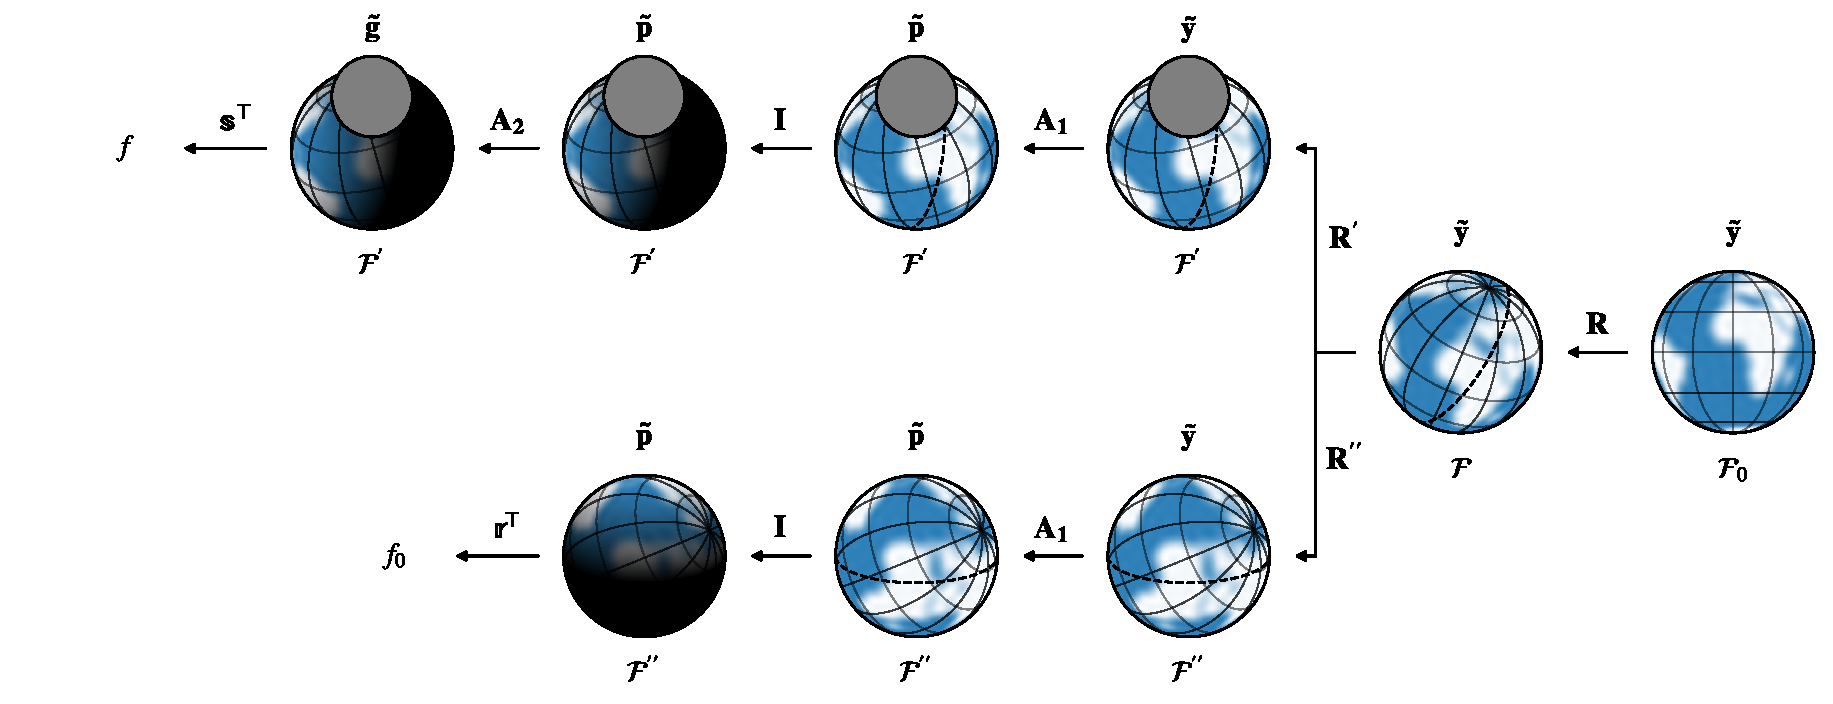
\includegraphics[width=\linewidth]{figures/frames.pdf}
        \oscaption{frames}{%
            How \starry computes the flux from a body in reflected light,
            tracking each of the linear transformations from the input map
            (far right) to the output (far left). The label below each map
            denotes the reference frame, while the label above
            each map denotes the basis in which the map is represented.
            Arrows indicate linear operations and are labeled accordingly.
            The upper branch corresponds to the unocculted case, while the
            lower branch corresponds to the case where an occultor is present.
            See text for details.
            \label{fig:frames}
        }
    \end{centering}
\end{figure}

We may now re-write Equations~(\ref{eq:rTA1Ry}) and (\ref{eq:sTARRy}) to
account for this illumination transformation. The flux outside of occultation
is now given by
%
\begin{align}
    \label{eq:rTIA1RRy}
    f = \rT \BF{I} \BF{A_1} \BF{R}'' \BF{R} \BF{y}
    \quad,
\end{align}
%
and the flux during an occultation by
%
\begin{align}
    \label{eq:sTA2IA1RRy}
    f = \sT \BF{A_2} \BF{I} \BF{A_1} \BF{R}' \BF{R} \BF{y}
    \quad.
\end{align}
%
Two notes about these equations. First, we introduced a new rotation matrix
$\BF{R}''$ in Equation~(\ref{eq:rTIA1RRy}), which rotates the problem so that
the semi-major axis of the terminator is aligned with the $x$-axis; as will
become clear in \S\ref{sec:case-0} below, this greatly simplifies the
integration step. Second, in the derivation of Equation~(\ref{eq:sTA2IA1RRy})
we used the fact that $\BF{A} = \BF{A_2} \BF{A_1}$
\citep[c.f. Equation~14 in][]{Luger2019}, where $\BF{A_1}$ transforms from
the spherical harmonic basis $\by$ to the polynomial basis $\bp$, and
$\BF{A_2}$ transforms from $\bp$ to the Green's basis $\bg$.

Figure~\ref{fig:frames} summarizes the transformations involved in the two
equations above. Starting on the right with a map vector $\BF{y}$ in
the spherical harmonic basis $\by$, defined in some observer-independent frame
$\mathcal{F}_0$, we first rotate it via $\BF{R}$ to the sky frame
$\mathcal{F}_\mathrm{sky}$, in which orientation the body is viewed by the
observer. If there is no occultation (upper branch of the figure), we then
rotate the map once more via $\BF{R}''$ to the integration frame
$\mathcal{F}_\mathrm{int}$, in which the terminator is parallel to the
$x$-axis. We then apply $\BF{A_1}$ to change basis to $\bp$, apply the
illumination transform $\BF{I}$, and finally dot in the solutions to the
surface integrals $\rT$. If, on the other hand, an occultor is present,
we rotate the map from $\mathcal{F}_\mathrm{sky}$ via $\BF{R}'$ to the frame
$\mathcal{F}_\mathrm{greens}$, in which the occultor lies along the
$+y$-axis. We then apply $\BF{A_1}$ to change basis to $\bp$ and $\BF{I}$
to weight the map by the illumination as above. Finally, we change basis
via $\BF{A_2}$ to the Green's basis, in which we compute and dot the
integrals $\sT$.

In \citet{Luger2019}, the crux of the problem was to compute the terms in the
vectors $\sT$ and $\rT$, which are surface integrals over
the region of the body that is visible to the observer
(see Figure 2 in that paper). Here, these integrals are significantly
more difficult, because they involve not only integration along the
limb of the body and of a possible occultor, but also along the
elliptical day/night terminator.

\begin{figure}[t!]
    \begin{centering}
        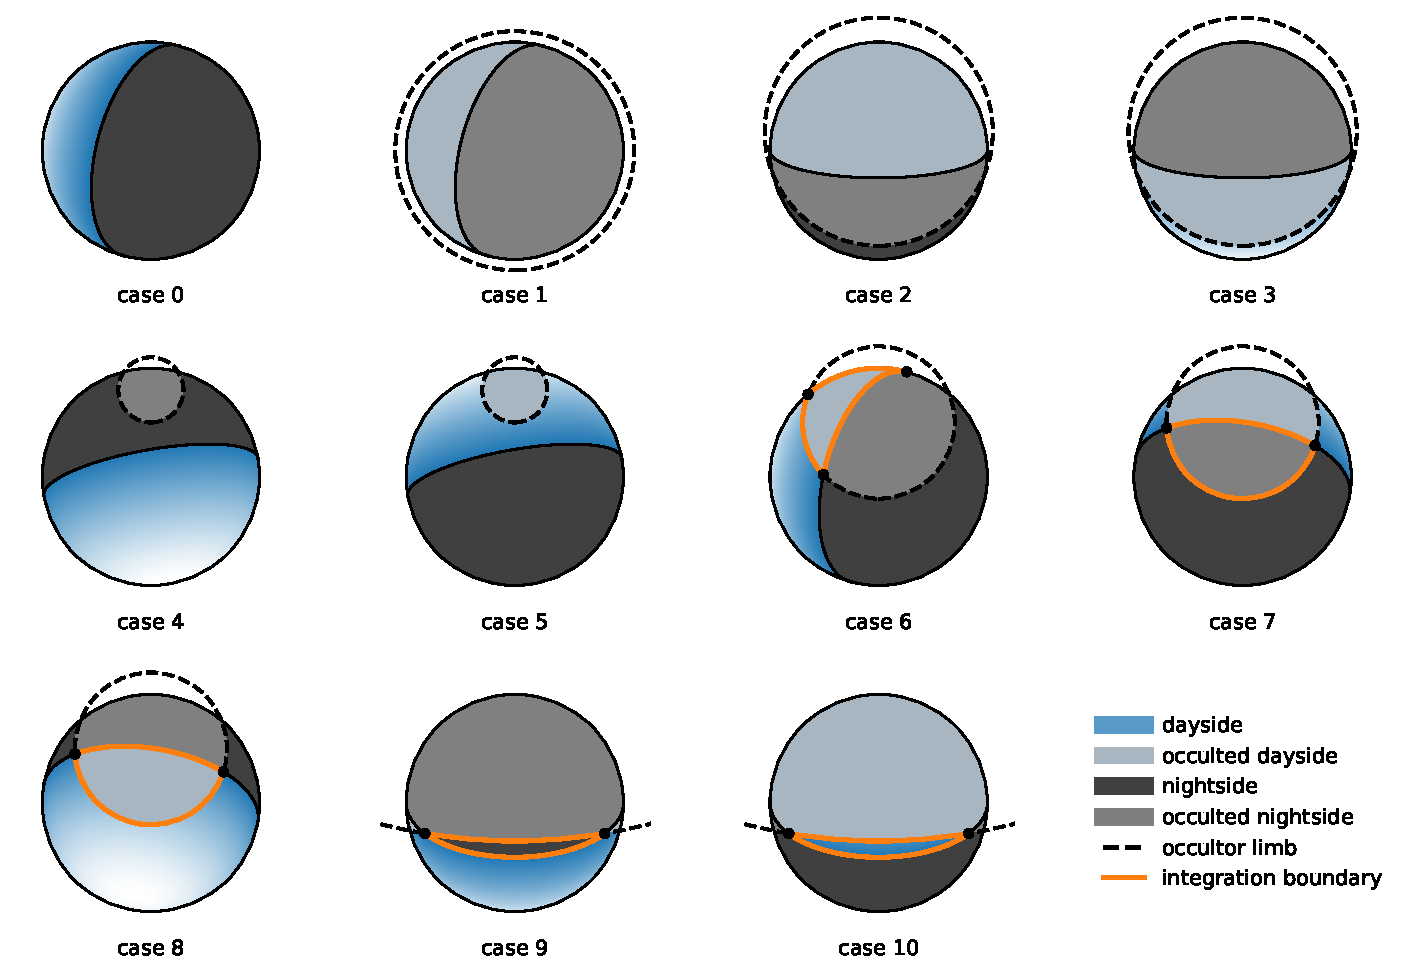
\includegraphics[width=\linewidth]{figures/cases.pdf}
        \oscaption{cases}{%
            The eight families of cases of occultations in reflected light.
            In these figures, the body with the solid outline
            is the one whose flux we are interested in, and the body with the
            dashed outline is the occultor.
            The night side of the occulted body is colored
            black (dark grey if occulted), and the dayside is colored blue
            (light grey if occulted).
            The cases in the top row involve
            configurations in which the limb of the occultor does not intersect
            with the terminator at any point, so the visible flux may be
            computed in terms of classical \starry integrals. The remaining
            cases require integration along the red boundary (the curves
            $\mathcal{P}$, $\mathcal{T}$, and $\mathcal{Q}$ of
            \S\ref{sec:cases-5-8}), which
            include the terminator. These involve the evaluation of incomplete
            elliptic integrals and are derived below.
            \label{fig:cases}
        }
    \end{centering}
\end{figure}

%

\subsection{Problem Setup}
\label{sec:setup}
%

Figure~\ref{fig:cases} shows the
eight families of cases involving an occultation of an illuminated body by
a spherical occultor. Each of these cases correspond to distinct ways in
which the limb of the occultor can intersect with the limb of the occulted
body and its terminator; together, these cases encompass all possible
occultation configurations, for any illumination angle, occultor size, and
occultor position. In the next three sections, we present the solution for the
$\sT$, and hence for the total visible flux, for each of these cases.

\section{The Solution}
\label{sec:solution}
%
\subsection{Case 0}
\label{sec:case-0}
%
Before we tackle configurations involving occultations, we must address the
simpler problem of computing the total visible flux from an unocculted
body in reflected light (see Figure~\ref{fig:illum}). This problem was
originally solved by \citet{Haggard2018} and subsequently adapted to the
\starry formalism in \citet{Luger2019b}, but for completeness we present
the detailed solution in Appendix~\ref{app:case0}. We will refer to the
solution vector for this case as $\sT_0$ (Equation~\ref{eq:sT0}).

\subsection{Cases 1--4}
\label{sec:cases-1-4}
%
Cases 1--4 (see Figure~\ref{fig:cases}) involve configurations in which the
occultor does not intersect with
the terminator of the occulted body, and are therefore fairly
straightforward to solve.
%
Case 1 corresponds to any complete occultation of the body, so its
solution vector is trivial:
%
\begin{align}
    \label{eq:sT1}
    \sT_1 = \BS{0}
    \quad.
\end{align}
%
Case 2 involves any occultation in which the occultor blocks \emph{only} the
night side of the body (regardless of whether or not it intersects with the
limb of the body). Since the night side intensity is zero everywhere, this case
is also trivial, as the integration is the same as in case 0:
%
\begin{align}
    \label{eq:sT2}
    \sT_2 = \sT_0(b, \theta)
    \quad.
\end{align}
%
Case 3 corresponds to occultations in which the occultor blocks \emph{all} of
the night side of the body and \emph{some} of the day side. In this
configuration, the unocculted part of the disk consists only of dayside.
Since we have no intersections with the terminator to worry about,
we may compute the total flux using the \starry formalism from
\citet{Luger2019}, provided we weight the intensity map by the illumination
field:
%
\begin{align}
    \label{eq:sT3}
    \sT_3 = \sT_\star(b_o, r_o) \BS{\Psi}(b, \theta, d_s)
    \quad,
\end{align}
%
where $\sT_\star$ is the usual \starry solution vector
\citep[Equation~26 in][]{Luger2019} and $\BS{\Psi}$ is an illumination
matrix (Appendix~\ref{app:case3}).
%
Finally, case 4 involves any occultation in which the occultor blocks
\emph{only} the day side of the body (regardless of whether or not it
intersects with the limb).
%
\begin{align}
    \label{eq:sT4}
    \sT_4 = \sT_\star(b_o, r_o) + \sT_0(-b, \theta + \pi)
    \quad.
\end{align}
%

% case 1: 0
% case 2: s0
% case 3: sTe * I
% case 4: sTe * I + ~sT0

\subsection{Cases 5--8}
\label{sec:cases-5-8}
%
Cases 5--8 (see Figure~\ref{fig:cases}, Figure~\ref{fig:geometry}).

% case 5: sT0 - sT0 * I
% case 6: (sTe + sT0) * I + ~sT0
% case 7: (sTe - sT0) * I
% case 8: sT0 * I

\begin{figure}[t!]
    \begin{centering}
        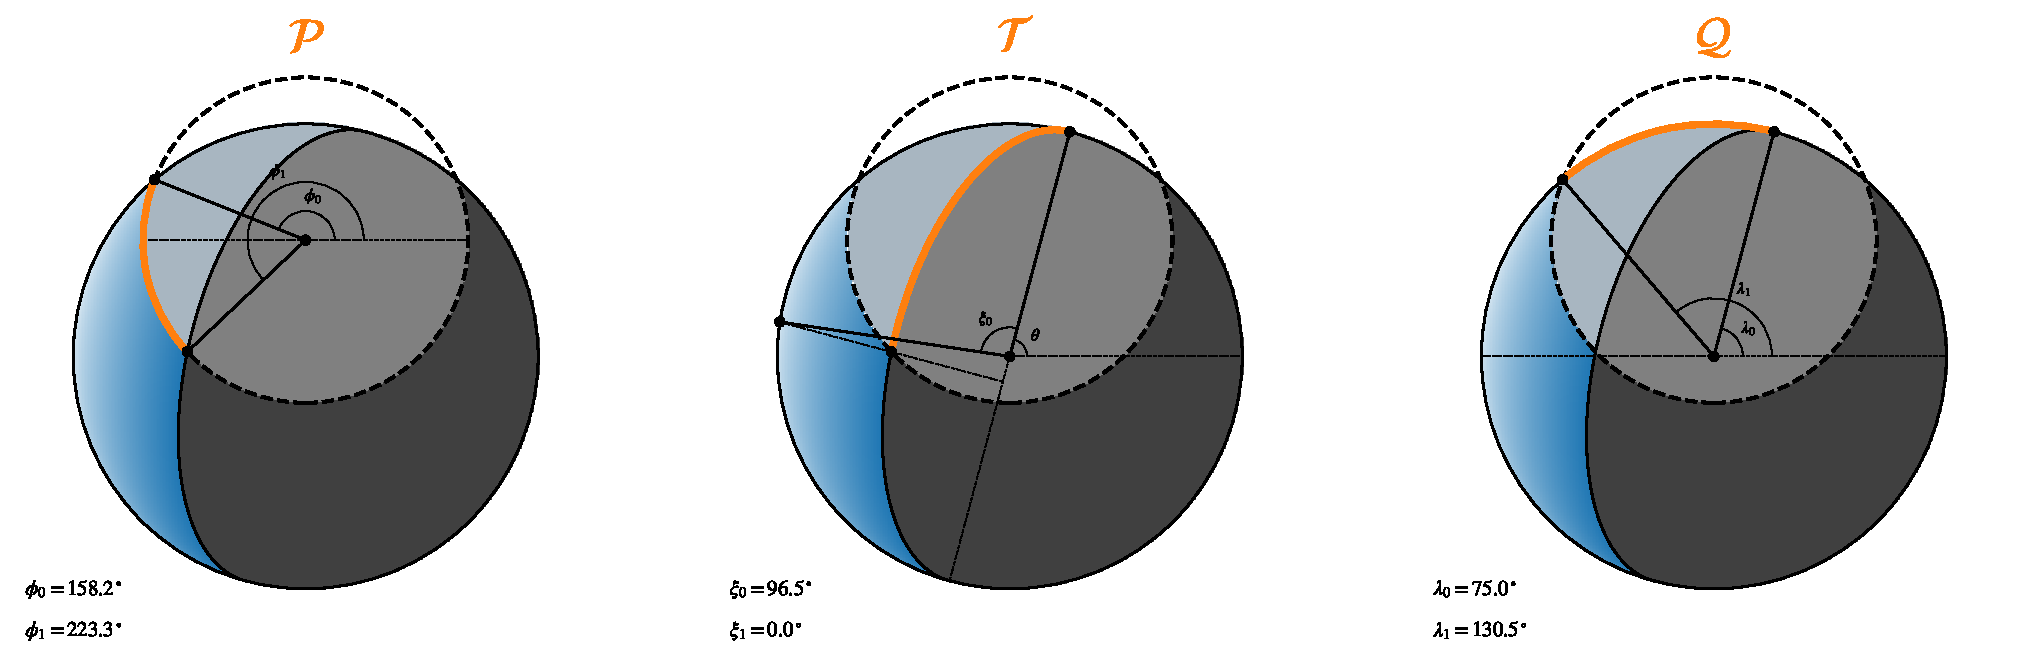
\includegraphics[width=\linewidth]{figures/geometry.pdf}
        \oscaption{geometry}{%
            Geometry of an occultation in reflected light, corresponding
            to case 5 in Figure~\ref{fig:cases}. The surface integral over
            the blue region is computed from the antiderivatives of the
            surface intensity map counter-clockwise along the boundary curves
            $\mathcal{P}$, $\mathcal{T}$, and $\mathcal{Q}$.
            \label{fig:geometry}
        }
    \end{centering}
\end{figure}


\section{Performance}
\label{sec:performance}
%
See Figure~\ref{fig:speed}.
%
\begin{figure}[h!]
    \begin{centering}
        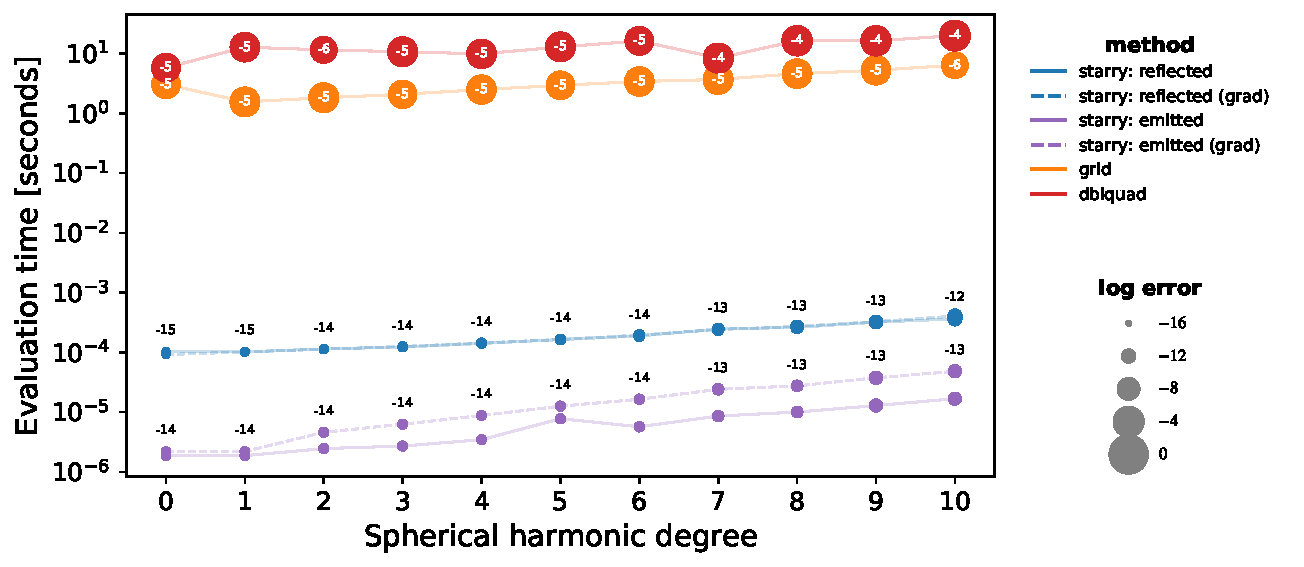
\includegraphics[width=\linewidth]{figures/speed.pdf}
        \oscaption{speed}{%
            Evaluation time for the starry algorithm.
            \label{fig:speed}
        }
    \end{centering}
\end{figure}

\appendix

\section{The \starry formalism}
\label{app:starry}
%
The basis $\bg$ is called the \emph{Green's basis}; its name
stems from the fact that its components have a structure that makes integration
by Green's theorem convenient. Its components were defined in
Equation~11 of \citet{Luger2019b}:
%
\begin{proof}{bg}
    \tilde{g}_{l,m} &=
    \begin{dcases}
        %
        \frac{\mu+2}{2}x^\frac{\mu}{2} y^\frac{\nu}{2}
         & \qquad \mu, \nu \, \mathrm{even}
        \\[1em]
        %
        z(x, y)
         & \qquad \mu = \nu = 1
        \\[1em]
        %
        3x^{l-2}yz(x, y)
         & \qquad \nu \, \mathrm{odd}, \,
        \mu = 1, \,
        \frac{\mu + \nu}{2} \, \mathrm{even}
        \\[1em]
        %
        z(x, y)
        \bigg(
        -x^{l-3} + x^{l-1} + 4x^{l-3}y^2
        \bigg)
         & \qquad \nu \, \mathrm{odd}, \,
        \mu = 1, \,
        \, \mathrm{odd}
        \\[1em]
        %
        z(x, y)
        \bigg(
        \frac{\mu-3}{2} x^\frac{\mu-5}{2} y^\frac{\nu-1}{2}
        \ - \
        \frac{\mu-3}{2} x^\frac{\mu-5}{2} y^\frac{\nu+3}{2}
        \\
        \qquad\qquad \ - \
        \frac{\mu+3}{2} x^\frac{\mu-1}{2} y^\frac{\nu-1}{2}
        \bigg)
         & \qquad \mathrm{otherwise}
        \quad,
    \end{dcases}
    \label{eq:bg}
\end{proof}
%
where $x$ and $y$ are the Cartesian coordinates on the surface
of the projected
disk of the body, with $z(x, y) = \sqrt{1 - x^2 - y^2}$, and
%
\begin{align}
    \label{eq:munu}
    \mu & = l - m
    \nonumber     \\
    \nu & = l + m
    \quad.
\end{align}
%
The vector $\bg$ is ordered such that
the component at index $n$ is $\tilde{g}_{l,m}$, with
%
\begin{align}
    \label{eq:lm}
    l & = \floor*{\sqrt{n}} \nonumber \\
    m & = n - l^2 - l
    \quad.
\end{align}
%
Finally, the rotation matrix $\BF{R} = \BF{R}(i, \lambda, \vartheta)$
rotates the body to the correct orientation on the sky given its
inclination $i$, obliquity $\lambda$, and rotational phase $\vartheta$,
while $\BF{R}'$ rotates the body on the plane
of the sky into the frame $\mathcal{F}'$ in which the integration is
actually performed, with the occultor along the $+y$-axis.
For more information on all of these terms, the reader is referred to
\citet{Luger2019}.

\section{Case 0}
\label{app:case0}
%
Our task is to compute the solution vector for this
configuration, which we will denote $\BF{s}^\top_0$.
Since in this case there is no occultor, it is
more convenient to perform the integration in a frame $\mathcal{F}''$ where the
semi-major axis of the terminator is aligned with the $x$-axis
(see Figure~\ref{fig:illum}); let us denote the matrix that rotates us
from $\mathcal{F}'$ to $\mathcal{F}''$ as $\BF{R}''$.
It is also far easier to perform the integration
in the \emph{polynomial basis} $\bp$
\citep[Equation 7 in][]{Luger2019}:
%
\begin{align}
    \tilde{p}_{l,m}(x, y) & =
    \begin{dcases}
        x^\frac{\mu}{2} y^\frac{\nu}{2}
         & \qquad \mu, \nu \, \mathrm{even}
        \\[1em]
        x^\frac{\mu-1}{2} y^\frac{\nu-1}{2} z(x, y)
         & \qquad \mathrm{otherwise} \quad,
    \end{dcases}
\end{align}
%
where $\bp$ is again ordered such that the component at
index $n$ is $\tilde{p}_{l,m}$, with $l$ and $m$ given by
Equation~(\ref{eq:lm}).
Now, if $\BF{r}^\top$ is the solution to the surface integrals in the
polynomial basis in $\mathcal{F}''$,
we may compute the desired solution vector in the Green's basis from
%
\begin{align}
    \label{eq:sT0}
    \BF{s}^\top_0 & = \BF{r}^\top \BF{A_1} \BF{R}'' \BF{A}^{-1}
    \quad,
\end{align}
%
where $\BF{A_1}$ \citep[Equation B11 in][]{Luger2019}
transforms the solution into the spherical harmonic basis so it can
be rotated out of the integration frame $\mathcal{F}''$ via $\BF{R}''$, and
$\BF{A}^{-1}$ \citep[Equation B13 in][]{Luger2019} transforms the
result into the Green's basis (in which $\sT$ is defined).

Our task is thus to compute $\BF{r}^\top$.
In frame $\mathcal{F}''$, the body sits at the origin and is
illuminated by a point source in the
$y-z$ plane at coordinates $(0, y_s, z_s)$ as in Figure~\ref{fig:illum}.
The day/night terminator is a half-ellipse whose semi-major axis
is unity and is aligned with the $x$-axis. The semi-minor axis is given
by $b = -\nicefrac{z_s}{\sqrt{y_s^2 + z_s^2}}$, where $b > 0$ corresponds to
a half-ellipse that is concave down and $b < 0$ to one that is concave up.
It is straightforward to show
that the illumination at a point $(x, y)$ on the projected disk is
given by
%
\begin{proof}{}
    \Psi(b; x, y) & =
    \begin{dcases}
        b_cy - bz(x, y) &
        \quad\quad\quad\quad\quad\quad\quad\quad\quad\quad
        y \geq b \sqrt{1 - x^2}
        \\
        0               &
        \quad\quad\quad\quad\quad\quad\quad\quad\quad\quad
        \mathrm{otherwise}
    \end{dcases}
    \quad ,
    \label{eq:illum}
\end{proof}
%
where $b_c = \sqrt{1 - b^2}$.
%
The elements of the solution vector may then be computed from
%
\begin{align}
    \label{eq:rT}
    r_{l, m}(b) & =
    \int_{-1}^{1}
    \int_{b\sqrt{1 - x^2}}^{\sqrt{1 - x^2}}
    \tilde{p}_{n(\mu,\nu)}(x, y)
    \Psi(b; x, y)
    \ \dd y \ \dd x
    \quad.
\end{align}
%
This is the integral of the illumination-weighted intensity of each
term in the polynomial basis over the projected visible dayside of the
body.
%
Equation~(\ref{eq:rT}) may be solved analytically in terms of purely
trigonometric and algebraic functions of $b$:
%
\begin{proof}{}
    \label{eq:rTsoln}
    r_{l, m}(b) & =
    \begin{cases}
        \frac{b_c\left(1 - b^{\frac{\nu + 4}{2}}\right)}{2}
        J_{\frac{\mu}{2}, \frac{\nu + 2}{2}} -
        b I_\frac{\nu}{2}(b) K_{\frac{\mu}{2}, \frac{\nu}{2}}
        %
         &
        %
        \qquad
        \mu, \nu \ \mathrm{even}
        %
        \\[1em]
        %
        b_c
        I_{\frac{\nu + 1}{2}}(b) K_{\frac{\mu - 1}{2}, \frac{\nu + 1}{2}}
        %
        \\[0.5em]
        \qquad
        %
        - \frac{b}{2} \bigg\{
        \left(1 - b^{\frac{\nu + 1}{2}}\right)
        \left(
        J_{\frac{\mu - 1}{2}, \frac{\nu - 1}{2}} -
        J_{\frac{\mu + 3}{2}, \frac{\nu - 1}{2}}
        \right)
        \\[0.5em]
        \qquad\qquad
        -
        \left(1 - b^{\frac{\nu + 5}{2}}\right)
        J_{\frac{\mu - 1}{2}, \frac{\nu + 3}{2}}
        \bigg\}
        %
         &
        %
        \qquad
        \mathrm{otherwise}
        %
    \end{cases}
\end{proof}
%
where
%
\begin{proof}{}
    \label{eq:IJK}
    I_{j}(b) &= \int_b^1 a^j \sqrt{1 - a^2} \dd a
    \nonumber \\
    %
    J_{i,j} &=
    \frac{
        \Gamma\left(\frac{i + 1}{2}\right)
        \Gamma\left(\frac{j + 1}{2}\right)
    }
    {
        \Gamma\left(\frac{i + j + 4}{2}\right)
    }
    %
    \nonumber \\
    %
    K_{i,j} &=
    \frac{
        \Gamma\left(\frac{i + 1}{2}\right)
        \Gamma\left(\frac{j + 4}{2}\right)
    }
    {
        \Gamma\left(\frac{i + j + 5}{2}\right)
    }
    \quad.
\end{proof}
%
Given initial conditions
%
\\[1em]
\begin{minipage}{.33\linewidth}
    \begin{align}
        I_{0}(b) & = \frac{\arccos(b) - bb_c}{2}
        %
        \nonumber                                \\
        %
        I_{1}(b) & = \frac{b_c^3}{3}
        %
        \nonumber
    \end{align}
\end{minipage}%
\begin{minipage}{.32\linewidth}
    \begin{align}
        J_{0,0} & = \pi
        %
        \nonumber               \\
        %
        J_{0,1} & = \frac{4}{3}
        %
        \nonumber
    \end{align}
\end{minipage}%
\begin{minipage}{.33\linewidth}
    \begin{proof}{}
        \label{eq:IJK0}
        K_{0,0} &= \frac{4}{3}
        %
        \nonumber \\
        K_{0,1} &= \frac{3\pi}{8}
    \end{proof}
\end{minipage}
\\[1em]
%
we may compute all higher order terms from the recurrence relations
%
\begin{proof}{}
    \label{eq:IJKrec}
    I_{j}(b) &= \frac{b^n b_c^3 + (j - 1) I_{j - 2}(b)}{j + 2}
    %
    \nonumber \\
    %
    J_{0,j} &= \left(\frac{j - 1}{j + 2}\right) J_{0,j-2}
    %
    \nonumber \\
    %
    K_{0,j} &= \left(\frac{j + 2}{j + 3}\right) K_{0,j-2}
    %
    \nonumber \\
    %
    J_{i,j} &= \left(\frac{i - 1}{i + j + 2}\right) J_{i-2,j}
    %
    \nonumber \\
    %
    K_{i,j} &= \left(\frac{i - 1}{i + j + 3}\right) K_{i-2,j}
    \quad.
\end{proof}

\section{Case 3}
\label{app:case3}
Hello.

\section{Case 4}
\label{app:case4}
Hello.

\section{Cases 5--8}
\label{app:cases-5-8}
Hello.

As in \citet{Luger2019}, the elements of the solution vector $\mathbf{s}^\top$
are given by the line integral
%
\begin{align}
    \label{eq:s}
    s_{n(\mu,\nu)} = \oint \mathbf{G}_{\mu,\nu} \cdot \dd\mathbf{r}
\end{align}
%
where
%
\begin{align}
    \label{eq:G}
    \BF{G}_{\mu,\nu} (x, y) & =
    \begin{dcases}
        %
        x^{\frac{\mu + 2}{2}}
        y^{\frac{\nu}{2}}
        \,\yhat
         & \qquad \mu, \nu \, \mathrm{even}
        \\[1em]
        %
        \frac{1-z(x, y)^3}{3(1-z(x, y)^2)}\bigg(-y \, \xhat + x \, \yhat\bigg)
         & \qquad \mu = \nu = 1
        \\[1em]
        %
        x^{l-2}
        z(x, y)^3
        \,\xhat
         & \qquad \nu \, \mathrm{odd}, \,
        \mu = 1, \,
        \frac{\mu + \nu}{2} \, \mathrm{even}
        \\[1em]
        %
        x^{l-3}
        y
        z(x, y)^3
        \,\xhat
         & \qquad \nu \, \mathrm{odd}, \,
        \mu = 1, \,
        \frac{\mu + \nu}{2} \, \mathrm{odd}
        \\[1em]
        %
        x^{\frac{\mu-3}{2}}
        y^{\frac{\nu-1}{2}}
        z(x, y)^3
        \,\yhat
         & \qquad \mathrm{otherwise,}
    \end{dcases}
\end{align}
%
and
%
\begin{align}
    \dd \BF{r} & = -r \sin\varphi \, \dd \varphi \, \xhat +
    r \cos\varphi \, \dd \varphi \, \yhat
    \quad,
\end{align}
%
where $\varphi = \varphi(x, y)$ is the parametrized angle along the
arc of integration. Generally, there are at most three arcs bounding a given
closed surface of integration, which we will denote $\mathcal{P}$,
$\mathcal{Q}$, and $\mathcal{T}$. These are shown for a typical
occultor-occulted configuration in Figure~\ref{fig:geometry}.

\subsection{Definitions}
%
Define the pairwise difference operator
%
\begin{align}
    \label{eq:pairdiff}
    \Delta \BS{v} \equiv \sum_{i=0}^{\frac{N - 1}{2}}
    \left( v_{2i + 1} - v_{2i} \right)
\end{align}
%
which sums the difference of successive pairs of values in
an array $\BS{v} = \{ v_0, v_1, v_2, v_3, {\cdot\cdot\cdot}, v_N\}$.

Define the quantity
%
\begin{align}
    \label{eq:q}
    \BS{q}(k^2, \bkappa) = \sqrt{1 - \frac{\sinhalfkap[2]}{k^2}}
    \quad.
\end{align}

\subsection{$\mathcal{H}_{u,v}$}
%
The function $\mathcal{H}_{u,v}$ is given by
%
\begin{align}
    \label{eq:H}
    \mathcal{H}_{u,v}(\blambda) & =
    \lamint{
        \cos^u\varphi
        \sin^v\varphi
    }
    \quad.
\end{align}
%
The integral in this expression is the same as that in Equation (D27)
of \citet{Luger2019}, except for a change in the limits of integration.
We can compute this integral recursively given four lower boundary conditions:
%
\begin{proof}{H}
    \label{eq:Hlower}
    \mathcal{H}_{0,0}(\blambda) &= \Delta \blambda
    %
    \nonumber \\
    %
    \mathcal{H}_{1,0}(\blambda) &= \Delta \sin\blambda
    %
    \nonumber \\
    %
    \mathcal{H}_{0,1}(\blambda) &= -\Delta \cos\blambda
    %
    \nonumber \\
    %
    \mathcal{H}_{1,1}(\blambda) &= -\frac{\Delta\cos^2\blambda}{2}
    %
    \quad.
\end{proof}
%
The remaining terms may be computed by upward recursion using the
relations
%
\begin{proof}{H}
    \label{eq:Hrec1}
    \mathcal{H}_{u,v}(\blambda) &=
    \frac{
        -\Delta \left(
        \cos^{u + 1} \blambda
        \sin^{v - 1} \blambda
        \right)
        +(v - 1)\mathcal{H}_{u,v - 2}(\blambda)
    }{u + v}
\end{proof}
%
for $u < 2, v \ge 2$ and
%
\begin{proof}{H}
    \label{eq:Hrec2}
    \mathcal{H}_{u,v}(\blambda) &=
    \frac{
        \Delta \left(
        \cos^{u - 1} \blambda
        \sin^{v + 1} \blambda
        \right)
        + (u - 1)\mathcal{H}_{u - 2,v}(\blambda)
    }{u + v}
\end{proof}
%
for all remaining terms.

\subsection{$\mathcal{T}_{2}$}
%
The function $\mathcal{T}_{2}$ is given by
%
\begin{align}
    \label{eq:T2}
    \mathcal{T}_{2}(b, \bxi) & = ?
    \quad.
\end{align}

\begin{proof}{}
    \mathcal{T}_{2}(b, \bxi) &= -\sgn(b) \Delta \BS{f}(b, \bxi)
\end{proof}
%
where
%
\begin{proof}{}
    \begin{split}
        f_i(b, \xi_i) =
        \frac{1}{3}\scalebox{1.4}{\Bigg(}
        &\arctan\left( \frac{|b|\sin\xi_i}{\cos\xi_i} \right)
        %
        \\
        %
        &- \sgn\left({\sin\xi_i}\right)
        \left(
        \arctan
        \left(
            \frac{
                \left(\frac{\sin\xi_i}{1 + \cos\xi_i}\right)^2 + 2 b^2 - 1
            }{2 |b| \sqrt{1 - b^2}}
            \right)
        + |b| \sqrt{1 - b^2} \cos\xi_i
        \right)
        %
        \\
        %
        &+ \phi(b, \xi_i)
        \scalebox{1.4}{\Bigg)}
    \end{split}
\end{proof}
%
and
%
\begin{proof}{}
    \phi(b, \xi_i) & =
    \begin{cases}
        0                          & \qquad 0 \leq \xi_i < \frac{\pi}{2}     \\
        \pi                        & \qquad \frac{\pi}{2} \leq \xi_i < \pi   \\
        2 |b| \sqrt{1 - b^2}       & \qquad \pi < \xi_i \leq \frac{3\pi}{2}  \\
        \pi + 2 |b| \sqrt{1 - b^2} & \qquad \frac{3\pi}{2} \leq \xi_i < 2\pi
        \quad.
    \end{cases}
\end{proof}

\subsection{$\mathcal{U}_v$}
%
The function $\mathcal{U}_v$ is given by
%
\begin{align}
    \label{eq:U}
    \mathcal{U}_v(\bkappa) =
    \kapint{\cos\varphi\sin^{2v}\varphi}
    \quad.
\end{align}
%
This integral has an analytic solution for all $v$:
%
\begin{proof}{U}
    \label{eq:Usol}
    \mathcal{U}_v(\bkappa) &= \frac{\Delta \sinhalfkap[v+1]}{v + 1}
    \quad.
\end{proof}
%

\subsection{$\mathcal{I}_v$}
%
The function $\mathcal{I}_v$ is given by
%
\begin{align}
    \label{eq:I}
    \mathcal{I}_v(\bkappa) & =
    \kapint{\sinhalfkap[2v]}
    \quad.
\end{align}
%
The integral in this expression is the same as that in Equation (D38)
of \citet{Luger2019}, except for a change in the limits of integration.
As in \citet{Luger2019}, we can compute this integral recursively given
a trivial lower boundary condition:
%
\begin{proof}{I}
    \label{eq:Irec}
    \mathcal{I}_0(\bkappa) &=
    \frac{\Delta \bkappa}{2}
    %
    \nonumber \\
    %
    \mathcal{I}_v(\bkappa) &=
    \frac{1}{2v}
    \bigg(
    (2v - 1) \mathcal{I}_{v-1}(\bkappa) -
    \Delta \left(\sinhalfkap[2v - 1]\coshalfkap\right)
    \bigg)
\end{proof}
%
where the last expression is valid for all $v > 0$. We find that this algorithm
is generally stable, except when $\sin\left(\frac{\bkappa}{2}\right)$ is small.
In that limit, we evaluate $\mathcal{I}_N(\bkappa)$ by numerical integration of
Equation~(\ref{eq:I}) using Gauss-Legendre quadrature with \STARRYQUADPOINTS
points. We then recurse downward by substituting $v \rightarrow v + 1$ in
Equation~(\ref{eq:Irec}) and solving for $\mathcal{I}_v(\bkappa)$.

\subsection{$\mathcal{J}_v$}
%
The function $\mathcal{J}_v$ is given by
%
\begin{align}
    \label{eq:J}
    \mathcal{J}_v(k^2, \bkappa) =
    \kapint{
        \sin^{2v}\varphi
        \left(1 - \frac{\sin^2\varphi}{k^2}\right)^\frac{3}{2}
    }
    \quad.
\end{align}
%
The integral in this expression is again the same as that in Equation (D39)
of \citet{Luger2019}, except for a change in the limits of integration.
In that paper, we computed all terms
$\{ \mathcal{J}_0, {\cdot\cdot\cdot}, \mathcal{J}_\vmax \}$ from a three-term
recurrence relation and two boundary conditions. In the case of upward
recursion, the boundary conditions $\mathcal{J}_0$ and $\mathcal{J}_1$ were
computed analytically from the complete elliptic integrals $K(k^2)$
and $E(k^2)$. In cases where upward recursion was not numerically stable, we
evaluated $\mathcal{J}_\vmax$ and $\mathcal{J}_{\vmax-1}$
via a quickly convergent series expansion and recursed downward.

In order to solve Equation~(\ref{eq:J}), it is possible to
replace the complete elliptic integrals $K(k^2)$ and $E(k^2)$ in the lower
boundary conditions \citep[Equation D46 in ][]{Luger2019} with the
incomplete elliptic integrals $F(k^2, \kappa)$ and $E(k^2, \kappa)$,
then use the same upward
recursion relation to obtain analytic solutions for all $\mathcal{J}_v$:
%
\begin{proof}{J}
    \label{eq:Jrec}
    \mathcal{J}_0(k^2, \bkappa) &=
    \frac{1}{3} \bigg(
    2 \left(2 - \frac{1}{k^2}\right) \DE +
    \left(\frac{1}{k^2} - 1\right) \DF +
    \Delta \BS{z}_0(k^2, \bkappa)
    \bigg)
    %
    \nonumber \\
    %
    \mathcal{J}_1(k^2, \bkappa) &=
    \frac{1}{15} \bigg(
    \left(-3 k^2 + 13 - \frac{8}{k^2}\right) \DE +
    \left(3 k^2 - 7 + \frac{4}{k^2}\right) \DF +
    \Delta \BS{z}_1(k^2, \bkappa)
    \bigg)
    %
    \nonumber \\
    %
    \mathcal{J}_v(k^2, \bkappa) &=
    \frac{1}{2v + 3}
    \bigg(
    2 \left( v + 1 + (v - 1) k^2 \right) \mathcal{J}_{v - 1} -
    (2v - 3) k^2 \mathcal{J}_{v - 2}
    + \Delta \BS{z}_v(k^2, \bkappa)
    \bigg)
\end{proof}
%
%
where the last expression is valid for all $v > 1$ and
%
\begin{proof}{J}
    \label{eq:Jrec_z}
    \BS{z}_0(k^2, \BS{\kappa}) & =
    \frac{
        \sinhalfkap
        \coshalfkap
        \BS{q}(k^2, \bkappa)
    }{
        k^2
    }
    %
    \nonumber\\
    %
    \BS{z}_1(k^2, \BS{\kappa}) & =
    \left(\left(3 \sinhalfkap[2] + 4\right) - 6k^2\right)
    \BS{z}_0(k^2, \BS{\kappa})
    %
    \nonumber\\
    %
    \BS{z}_v(k^2, \BS{\kappa}) & =
    k^2
    \sinhalfkap[2v - 3]
    \coshalfkap
    \BS{q}(k^2, \BS{\kappa})^5
    \quad.
\end{proof}
%
However, in practice we find that this procedure is even more numerically
unstable than it was in \citet{Luger2019}.
To address this, we express the recurrence structure of the problem as
a tridiagonal system with one lower boundary condition $\mathcal{J}_0$
and one upper boundary condition $\mathcal{J}_\vmax$:
%
\begin{proof}{J}
    \label{eq:Jtri}
    \begin{pmatrix}
        a_0 & 1   &     &        &         &         \\
        b_1 & a_1 & 1   &        &         &         \\
            & b_2 & a_2 & 1      &         &         \\
            &     & b_0 & a_3    & 1       &         \\
            &     &     & \ddots & \ddots  & \ddots  \\
            &     &     &        & b_\vmax & a_\vmax
    \end{pmatrix}
    \begin{pmatrix}
        \mathcal{J}_1   \\
        \mathcal{J}_2   \\
        \mathcal{J}_3   \\
        \mathcal{J}_4   \\
        \cdot\cdot\cdot \\
        \mathcal{J}_{\vmax-1}
    \end{pmatrix}
    =
    \begin{pmatrix}
        c_0 - b_0 \mathcal{J}_0 \\
        c_1                     \\
        c_2                     \\
        c_3                     \\
        \cdot\cdot\cdot         \\
        c_\vmax - \mathcal{J}_\vmax
    \end{pmatrix}
\end{proof}
%
where the recursion coefficients are given by
%
\begin{proof}{J}
    \label{eq:Jtri_coeffs}
    a_v(k) &= -2\frac{(v + 1) + (v - 1) k^2}{2v + 3} \nonumber \\
    b_v(k) &= \frac{(2v - 3) k^2}{2v + 3} \nonumber \\
    c_v(k^2, \bkappa) &= \Delta
    \bigg(
    \frac{
            \BS{z}_v(k^2, \BS{\kappa})
        }{
            2v + 3
        }
    \bigg)
    \quad.
\end{proof}
%
Solving this matrix system yields values for all
intermediate $\{ \mathcal{J}_1, {\cdot\cdot\cdot}, \mathcal{J}_{\vmax - 1} \}$.
While efficient algorithms exist for solving tridiagonal problems, we obtain
far better numerical stability by instead performing traditional LU
decomposition. We find that this algorithm is stable in all the regimes that we
tested.

We evaluate the upper boundary condition $\mathcal{J}_{\vmax}$ by numerical
integration of Equation~(\ref{eq:J}) via Gauss-Legendre quadrature with
\STARRYQUADPOINTS points. While the lower boundary condition may be computed
analytically from Equation~(\ref{eq:Jrec}),
in practice we achieve better precision via numerical
integration (as above), with negligible effects on computational performance.

\subsection{$\mathcal{W}_n$}
%
The function $\mathcal{W}_n$ is given by
%
\begin{align}
    \label{eq:W}
    % TODO
    \mathcal{W}_n = \int
\end{align}
%
This integral has a closed-form solution:
%
\begin{proof}{}
    \label{eq:Wsol}
    \mathcal{W}_n =
    \frac{\sin^{2n + 2}\left(\frac{\bkappa}{2}\right)}{2n + 5}
    \left(
    \frac{3}{n+1}
        {_2F_1}\left(-\frac{1}{2}, n + 1; n + 2; 1 - q^2\right) + 2 q^3
    \right)
\end{proof}
%
where ${_2F_1}(a, b; c; z)$ is the Gauss hypergeometric function.


% by either upward recursion (stable for |1 - q^2| > 1/2) or downward
% recursion (always stable).

% Bibliography
\bibliography{bib}


\end{document}
